%% ================================================================
%%  Usability Report — Mejora de Goiko
%%  DIU2.Errores404 · Universidad de Granada · 2025/26
%%  Compilar con: xelatex report_goiko.tex (2 pasadas)
%% ================================================================
\documentclass[11pt,a4paper]{article}

%% ── FUENTES Y CODIFICACIÓN (XeLaTeX) ────────────────────────────
\usepackage{fontspec}
\setmainfont[
  BoldFont       = Lato-Bold,
  ItalicFont     = Lato-Italic,
  BoldItalicFont = Lato-BoldItalic
]{Lato-Regular}
\setsansfont{Lato}
\setmonofont[Scale=0.88]{TeX Gyre Cursor}

\usepackage{polyglossia}
\setmainlanguage{spanish}

%% ── GEOMETRÍA ───────────────────────────────────────────────────
\usepackage[
  a4paper,
  top=2.6cm, bottom=2.8cm,
  left=3.0cm, right=2.6cm,
  headheight=16pt
]{geometry}

%% ── COLORES ─────────────────────────────────────────────────────
\usepackage{xcolor}
\definecolor{coverdark}   {HTML}{0F1923}
\definecolor{primarydark} {HTML}{1A2332}
\definecolor{sectionblue} {HTML}{1C3557}
\definecolor{goikored}    {HTML}{C0392B}
\definecolor{accentred}   {HTML}{E74C3C}
\definecolor{lightbg}     {HTML}{F7F9FC}
\definecolor{tabhead}     {HTML}{1A2332}
\definecolor{roweven}     {HTML}{EEF2F7}
\definecolor{medgray}     {HTML}{5D6D7E}
\definecolor{lightgray}   {HTML}{ECF0F1}
\definecolor{okgreen}     {HTML}{1E8449}
\definecolor{warnamber}   {HTML}{D68910}
\definecolor{dangerred}   {HTML}{C0392B}

%% ── GRÁFICOS ────────────────────────────────────────────────────
\usepackage{graphicx}
\usepackage{float}
\usepackage{caption}
\usepackage{subcaption}
\graphicspath{{./}}

%% ── TABLAS ──────────────────────────────────────────────────────
\usepackage{booktabs}
\usepackage{tabularx}
\usepackage{array}
\usepackage{colortbl}
\usepackage{multirow}
\newcolumntype{L}[1]{>{\raggedright\arraybackslash}p{#1}}
\newcolumntype{C}[1]{>{\centering\arraybackslash}p{#1}}
\setlength{\tabcolsep}{7pt}
\renewcommand{\arraystretch}{1.4}

%% ── TIKZ ────────────────────────────────────────────────────────
\usepackage{tikz}
\usetikzlibrary{calc, positioning, shapes.geometric}

%% ── CABECERAS Y PIES ────────────────────────────────────────────
\usepackage{fancyhdr}
\pagestyle{fancy}
\fancyhf{}
\fancyhead[L]{\small\color{medgray}\textit{Usability Report — Mejora de Goiko}}
\fancyhead[R]{\small\color{medgray}\textit{DIU2.Errores404 · 2025/26}}
\fancyfoot[C]{\small\color{medgray}— \thepage\ —}
\renewcommand{\headrulewidth}{0.8pt}
\renewcommand{\headrule}{{\color{goikored}\hrule width\headwidth height 0.8pt}}
\renewcommand{\footrulewidth}{0pt}

%% ── SECCIONES ───────────────────────────────────────────────────
\usepackage{titlesec}

\titleformat{\section}
  {\Large\bfseries\color{primarydark}}
  {\colorbox{goikored}{\color{white}\hspace{5pt}\thesection\hspace{5pt}}}
  {9pt}
  {}
  [{\vspace{1pt}\color{primarydark}\titlerule[2pt]}]

\titleformat{\subsection}
  {\large\bfseries\color{sectionblue}}
  {\thesubsection\enspace}
  {0em}
  {}
  [{\vspace{-0.4ex}\color{goikored}\titlerule[1.5pt]}]

\titleformat{\subsubsection}
  {\normalsize\bfseries\color{primarydark}}
  {}
  {0em}
  {}

\titlespacing{\section}     {0pt}{1.8ex plus .4ex minus .2ex}{1ex plus .2ex}
\titlespacing{\subsection}  {0pt}{1.4ex plus .3ex minus .1ex}{0.5ex plus .1ex}
\titlespacing{\subsubsection}{0pt}{1ex plus .2ex minus .1ex}{0.3ex}

%% ── TABLA DE CONTENIDOS ─────────────────────────────────────────
\usepackage{titletoc}
\titlecontents{section}[1.5em]
  {\addvspace{4pt}\bfseries\color{primarydark}}
  {\contentslabel{1.5em}}
  {\hspace*{-1.5em}}
  {\hfill\color{goikored}\contentspage}
\titlecontents{subsection}[3.8em]
  {\addvspace{2pt}\small\color{sectionblue}}
  {\contentslabel{2.3em}}
  {\hspace*{-2.3em}}
  {\dotfill\small\color{medgray}\contentspage}

%% ── CAJAS ESPECIALES ────────────────────────────────────────────
\usepackage{tcolorbox}
\tcbuselibrary{skins, breakable, most}

\newtcolorbox{keybox}[1][Hallazgo Clave]{
  enhanced, breakable,
  colback  = goikored!7,
  colframe = goikored,
  coltitle = white,
  fonttitle= \bfseries,
  title    = #1,
  attach boxed title to top left = {yshift=-2.5mm, xshift=6mm},
  boxed title style = {colback=goikored, colframe=goikored, arc=3pt},
  arc = 3pt,
  leftrule = 5pt,
}

\newtcolorbox{infobox}{
  enhanced,
  colback  = sectionblue!7,
  colframe = sectionblue,
  leftrule = 5pt, toprule=0.5pt, bottomrule=0.5pt, rightrule=0.5pt,
  arc = 2pt,
}

%% ── LISTAS ──────────────────────────────────────────────────────
\usepackage{enumitem}
\setlist[itemize]  {leftmargin=1.6em, itemsep=2pt, topsep=4pt, parsep=0pt}
\setlist[enumerate]{leftmargin=1.6em, itemsep=2pt, topsep=4pt, parsep=0pt}

%% ── CAPTIONS ────────────────────────────────────────────────────
\captionsetup{
  font={small, color=medgray},
  labelfont={bf, color=primarydark},
  justification=centering,
  skip=5pt,
}

%% ── MISC ────────────────────────────────────────────────────────
\usepackage{microtype}
\usepackage{parskip}
\setlength{\parskip}{5pt plus 1pt}

\usepackage{hyperref}
\hypersetup{
  colorlinks = true,
  linkcolor  = primarydark,
  urlcolor   = sectionblue,
  pdftitle   = {Usability Report — Mejora de Goiko},
  pdfauthor  = {DIU2.Errores404},
  pdfsubject = {Usability Evaluation DIU 2025/26},
}

%% ================================================================
\begin{document}

%% ════════════════════════════════════════════════════════════════
%%  PORTADA
%% ════════════════════════════════════════════════════════════════
\begin{titlepage}
\newgeometry{margin=0pt}

\begin{tikzpicture}[remember picture, overlay]
  %% fondo total
  \fill[coverdark] (current page.north west) rectangle (current page.south east);
  %% banda roja superior
  \fill[goikored] ([yshift=0cm]current page.north west)
                  rectangle ([yshift=-1.4cm]current page.north east);
  %% anillos concéntricos en esquina inferior-derecha (lejos del texto)
  \fill[goikored!22] (current page.south east) circle(10cm);
  \fill[coverdark]   (current page.south east) circle(8cm);
  \fill[goikored!14] (current page.south east) circle(6cm);
  \fill[coverdark]   (current page.south east) circle(4.2cm);
  %% línea vertical acento izquierda
  \fill[goikored] ([xshift=2.4cm]current page.north west)
                  rectangle ([xshift=2.9cm]current page.south west);
  %% banda inferior oscura sobre los anillos
  \fill[primarydark!85] (current page.south west)
                        rectangle ([yshift=2.8cm]current page.south east);
\end{tikzpicture}

\begin{minipage}[t][26cm][t]{\textwidth}
  \vspace{4.2cm}
  \hspace{3.5cm}%
  \begin{minipage}{13.5cm}

    {\fontsize{8.5}{11}\selectfont\color{goikored}\bfseries\MakeUppercase{%
      Diseño de Interfaces de Usuario · Curso 2025/26}}

    \vspace{1cm}
    {\fontsize{42}{50}\selectfont\color{white}\bfseries Usability\\[0.15cm]Report}

    \vspace{0.4cm}
    {\color{goikored}\rule{9cm}{2.5pt}}
    \vspace{0.7cm}

    {\fontsize{14}{18}\selectfont\color{white!75!coverdark}%
      Evaluación de usabilidad del proyecto}

    \vspace{0.3cm}
    {\fontsize{24}{30}\selectfont\color{white}\bfseries Mejora de Goiko}

    \vspace{0.25cm}
    {\fontsize{11}{14}\selectfont\color{white!55!coverdark}
      \href{https://goikomejorado.surge.sh}{\color{goikored!80}goikomejorado.surge.sh}
      \enspace·\enspace
      \href{https://github.com/ClaudioDevv/UX\_CaseStudy}{\color{goikored!80}ClaudioDevv/UX\_CaseStudy}}

    \vspace{3cm}
    \begin{tikzpicture}
      \node[fill=goikored, rounded corners=5pt,
            inner xsep=12pt, inner ysep=7pt] {%
        \color{white}\bfseries\normalsize Caso B — Estudio A/B Testing
      };
    \end{tikzpicture}

    \vspace{3cm}
    {\fontsize{9}{12}\selectfont\color{white!60!coverdark} Informe elaborado por}
    \vspace{0.35cm}

    {\fontsize{18}{24}\selectfont\color{white}\bfseries Equipo DIU2.Errores404}

    \vspace{0.25cm}
    {\fontsize{11}{15}\selectfont\color{white!65!coverdark}%
      Julian Carrion Tovar \enspace·\enspace Miguel Angel Luque Gomez}

  \end{minipage}
\end{minipage}

\begin{tikzpicture}[remember picture, overlay]
  \node[anchor=south, yshift=0.9cm] at (current page.south) {
    \color{white!70!primarydark}\small
    Universidad de Granada \enspace·\enspace Mayo 2026
  };
\end{tikzpicture}

\restoregeometry
\end{titlepage}

%% ════════════════════════════════════════════════════════════════
%%  TABLA DE CONTENIDOS
%% ════════════════════════════════════════════════════════════════
\newpage
\setcounter{page}{1}
\pagestyle{fancy}

\begin{center}
  {\Large\bfseries\color{primarydark} Índice de Contenidos}
\end{center}
\vspace{0.3cm}
{\color{goikored}\rule{\textwidth}{1.5pt}}
\vspace{0.2cm}

\tableofcontents

\vspace{0.4cm}
{\color{lightgray}\rule{\textwidth}{0.5pt}}
\newpage

%% ════════════════════════════════════════════════════════════════
\section{Resumen Ejecutivo}
%% ════════════════════════════════════════════════════════════════

\subsection{Objetivo}

Evaluar la usabilidad del rediseño web del restaurante \textbf{Mejora de Goiko} (Caso B),
desarrollado por el equipo
\href{https://github.com/ClaudioDevv/UX\_CaseStudy}{ClaudioDevv/UX\_CaseStudy}.
El propósito del rediseño es modernizar la presencia digital de Goiko mejorando la navegación,
la búsqueda de restaurantes, el proceso de reserva \textit{online} y la visibilidad del menú.
La evaluación se enmarca en un estudio comparativo \textbf{A/B Testing} frente a la propuesta
NeoQarmita (Caso A), con el objetivo de identificar fortalezas y áreas de mejora antes de
una hipotética puesta en producción.

\subsection{Metodología}

Se ha empleado un enfoque mixto que combina cuatro técnicas complementarias:

\begin{itemize}
  \item \textbf{A/B Testing} con 5 usuarios reales asignados al Caso B —
        sesiones presenciales de 5 a 10 minutos.
  \item \textbf{Cuestionario SUS} (\textit{System Usability Scale}) de 10 ítems
        en escala Likert 1–5, administrado mediante Tally.so al finalizar la sesión.
  \item \textbf{Eye Tracking} con la herramienta GazeMapping sobre las pantallas
        principales del diseño, con Puntos de Interés (POI) definidos.
  \item \textbf{Auditoría de accesibilidad} automática con WAVE y Google Lighthouse
        (escritorio y móvil) según el marco \textbf{WCAG 2.1 nivel AA}.
\end{itemize}

\subsection{Principales Hallazgos}

\begin{enumerate}
  \item \textbf{Invisibilidad del CTA de reserva:} El botón principal de reserva en la
        \textit{Landing Page} no capta la atención del usuario. El Eye Tracking revela que
        el \textbf{100\%} de los usuarios ignoró el CTA en la exploración inicial —
        la atención se concentra en el hero y el logotipo, ignorando el elemento de
        conversión crítico.

  \item \textbf{Proceso de reserva excesivamente largo:} El formulario de pago y datos
        (78s de tiempo medio) es el cuello de botella principal. Los usuarios con menor
        competencia digital abandonaron parcialmente el flujo. La elección de salsas
        genera 9 clics medios, el valor más alto de todas las tareas.

  \item \textbf{Problemas estructurales de accesibilidad:} La web carece de encabezados
        semánticos (\texttt{<h1>}, \texttt{<h2>}) y de \textit{landmarks} de página,
        incumpliendo WCAG 2.1 AA. El LCP en móvil de 28,3 segundos supone una barrera
        de uso grave en conexiones estándar.
\end{enumerate}

\begin{keybox}[Resultado Global]
Puntuación SUS media de \textbf{62,0} (Grade D · Percentil 1º).
Categoría \textbf{«OK»} con aceptabilidad \textbf{Marginal} según Sauro \& Lewis.
El diseño es funcionalmente válido para perfiles técnicos, pero no supera el umbral
de «Aceptable» para el público general.
Se recomienda revisión de prioridad alta en el flujo de reserva, el CTA principal
y la estructura HTML antes de considerar el diseño listo para producción.
\end{keybox}

%% ════════════════════════════════════════════════════════════════
\section{Metodología y Reclutamiento}
%% ════════════════════════════════════════════════════════════════

\subsection{Perfil de los participantes}

Se ha realizado un estudio entre-sujetos con \textbf{5 usuarios} asignados al Caso B
(Mejora de Goiko). La muestra recoge un rango diverso de edades, niveles de competencia
digital y dispositivos de acceso.

\vspace{0.4em}
\begin{table}[H]
\centering
\caption{Participantes del Caso B — Mejora de Goiko}
\begin{tabularx}{\textwidth}{@{}
    C{1.9cm} C{1.5cm} L{2.8cm} C{1.6cm} C{2.2cm} C{2.2cm}@{}}
\toprule
\rowcolor{tabhead}
\color{white}\textbf{Usuario}     &
\color{white}\textbf{Sexo/Edad}   &
\color{white}\textbf{Ocupación}   &
\color{white}\textbf{Exp. TIC}    &
\color{white}\textbf{Personalidad}&
\color{white}\textbf{Plataforma}  \\
\midrule
P06 — Elena   & M / 24 & Estudiante    & Alta  & Comparativa & Portátil  \\
\rowcolor{roweven}
P07 — David   & H / 31 & Desarrollador & Alta  & Analítico   & Portátil  \\
P08 — Pilar   & M / 52 & Usuario final & Baja  & Cautelosa   & Tablet    \\
\rowcolor{roweven}
P09 — Roberto & H / 35 & Usuario final & Media & Práctico    & Sobremesa \\
P10 — Nadia   & M / 21 & Estudiante    & Media & Visual      & Móvil     \\
\bottomrule
\end{tabularx}
\end{table}

\begin{infobox}
\textbf{Edad media:} 32,6 años\enspace·\enspace
\textbf{Nivel digital:} Medio-Alto (2 Alta, 2 Media, 1 Baja)\enspace·\enspace
\textbf{Dispositivos:} 2 portátiles · 1 tablet · 1 sobremesa · 1 móvil
\end{infobox}

\textbf{Posibles situaciones conflictivas por usuario:}

\begin{itemize}
  \item \textbf{P06 Elena:} Puede comparar inconscientemente con otras webs de restaurantes.
  \item \textbf{P07 David:} Puede frustrarse si detecta problemas técnicos o de rendimiento.
  \item \textbf{P08 Pilar:} Puede abandonar el flujo de reserva si hay demasiados pasos.
  \item \textbf{P09 Roberto:} Puede tener dificultades si la búsqueda de restaurante no es intuitiva.
  \item \textbf{P10 Nadia:} Puede perder interés si la web no está optimizada para móvil.
\end{itemize}

\subsection{Escenario de la prueba}

Las sesiones se realizaron de forma \textbf{presencial} (5–10 minutos por usuario).
Se propusieron 4 tareas concretas sobre las pantallas principales:

\begin{enumerate}
  \item Localiza el restaurante Goiko más cercano a tu ubicación.
  \item Realiza una reserva \textit{online} para 3 personas esta noche.
  \item Consulta el menú y encuentra las opciones vegetarianas disponibles.
  \item Encuentra la vía de contacto para atención al cliente o redes sociales.
\end{enumerate}

Se anotó si el usuario completó la tarea sin ayuda, el tiempo empleado y el número de clics.
Al finalizar se administró el cuestionario SUS.

\subsection{Herramientas utilizadas}

\begin{table}[H]
\centering
\caption{Herramientas de evaluación empleadas}
\begin{tabularx}{\textwidth}{@{} L{4.5cm} X @{}}
\toprule
\rowcolor{tabhead}
\color{white}\textbf{Herramienta}         &
\color{white}\textbf{Propósito}           \\
\midrule
GazeMapping                 & Eye Tracking: generación de mapas de calor sobre pantallas fijas del diseño \\
\rowcolor{roweven}
FireShot (Chrome)           & Captura de las pantallas analizadas en Eye Tracking \\
Tally.so                    & Administración online del cuestionario SUS \\
\rowcolor{roweven}
SUS Tools (sus.tools)       & Cálculo de puntuación y etiqueta SUS individual \\
sus.mixality.de             & Análisis multivariable y comparativa A vs. B \\
\rowcolor{roweven}
WAVE                        & Auditoría automática de accesibilidad web \\
Google Lighthouse/PageSpeed & Auditoría de rendimiento, accesibilidad, SEO y buenas prácticas \\
\bottomrule
\end{tabularx}
\end{table}

%% ════════════════════════════════════════════════════════════════
\section{Resultados del Cuestionario SUS}
%% ════════════════════════════════════════════════════════════════

\subsection{Respuestas individuales por usuario}

\begin{table}[H]
\centering
\caption{Respuestas al cuestionario SUS — Caso B (escala Likert 1–5)}
\footnotesize
\begin{tabularx}{\textwidth}{@{} C{0.45cm} X C{0.75cm} C{0.75cm} C{0.75cm} C{0.75cm} C{0.75cm} @{}}
\toprule
\rowcolor{tabhead}
\color{white}\textbf{\#} &
\color{white}\textbf{Pregunta} &
\color{white}\textbf{P06} &
\color{white}\textbf{P07} &
\color{white}\textbf{P08} &
\color{white}\textbf{P09} &
\color{white}\textbf{P10} \\
\midrule
1  & Creo que me gustará visitar con frecuencia este website            & 4 & 3 & 3 & 4 & 4 \\
\rowcolor{roweven}
2  & Encontré el website innecesariamente complejo                      & 2 & 2 & 3 & 3 & 3 \\
3  & Pensé que era fácil utilizar este website                          & 4 & 4 & 3 & 3 & 3 \\
\rowcolor{roweven}
4  & Creo que necesitaría apoyo de un experto para recorrer el website  & 2 & 2 & 3 & 2 & 2 \\
5  & Encontré las funciones del website bastante bien integradas        & 4 & 3 & 2 & 4 & 3 \\
\rowcolor{roweven}
6  & Pensé que había demasiada inconsistencia en el website             & 2 & 3 & 3 & 2 & 3 \\
7  & Imagino que la mayoría aprenderían rápidamente a utilizarlo        & 4 & 4 & 3 & 4 & 4 \\
\rowcolor{roweven}
8  & Encontré el website muy grande al recorrerlo                       & 2 & 2 & 3 & 3 & 3 \\
9  & Me sentí muy confiado/a en el manejo del website                   & 3 & 4 & 3 & 3 & 3 \\
\rowcolor{roweven}
10 & Necesito aprender muchas cosas antes de manejarme en el website    & 2 & 2 & 3 & 2 & 3 \\
\bottomrule
\end{tabularx}
\end{table}

\subsection{Puntuaciones individuales y comparativa A vs. B}

\begin{table}[H]
\centering
\caption{Puntuaciones SUS — comparativa entre Caso A y Caso B}
\begin{tabularx}{\textwidth}{@{} L{4.2cm} C{1.8cm} C{2.8cm} L{4.5cm} @{}}
\toprule
\rowcolor{tabhead}
\color{white}\textbf{Usuario}         &
\color{white}\textbf{Caso}            &
\color{white}\textbf{Puntuación SUS}  &
\color{white}\textbf{Etiqueta}        \\
\midrule
P06 — Elena    & B & 72,5 & Good \\
\rowcolor{roweven}
P07 — David    & B & 67,5 & OK \\
P08 — Pilar    & B & \textcolor{dangerred}{\textbf{47,5}} & \textcolor{dangerred}{\textbf{Poor}} \\
\rowcolor{roweven}
P09 — Roberto  & B & 65,0 & OK \\
P10 — Nadia    & B & 57,5 & OK \\
\midrule
\rowcolor{goikored!18}
\textbf{Media Caso B}           & — & \textbf{62,0} & \textbf{OK / Marginal (Grade D)} \\
\rowcolor{okgreen!12}
\textit{Media Caso A (ref.)}    & — & \textit{73,0} & \textit{Good / Acceptable (Grade B)} \\
\bottomrule
\end{tabularx}
\end{table}

\subsection{Análisis multivariable}

\begin{figure}[H]
  \centering
  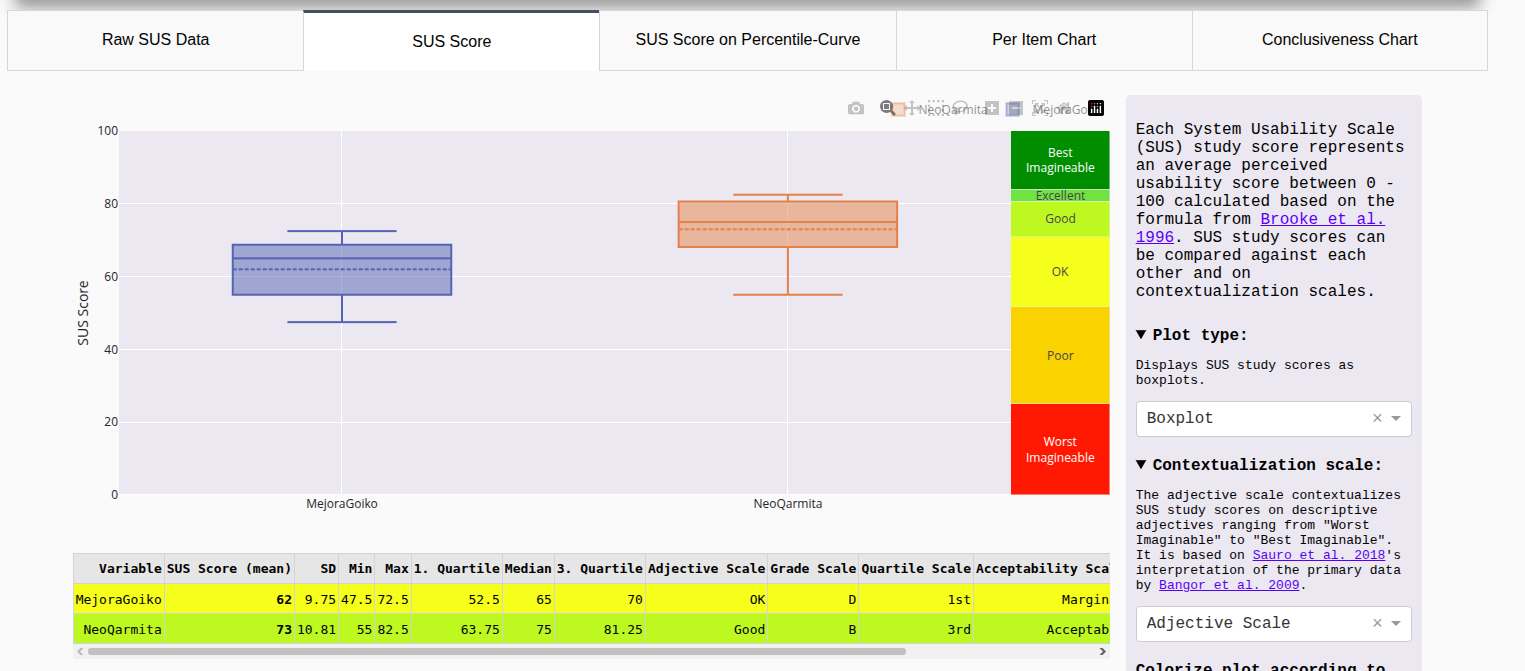
\includegraphics[width=0.82\textwidth]{sus1.png}
  \caption{Análisis SUS multivariable — Comparativa Caso A vs. Caso B (sus.mixality.de)}
\end{figure}

El análisis multivariable confirma que el Caso B (Mejora de Goiko) obtiene una media de
\textbf{62,0} (SD 9,75), situándose en la categoría \textbf{OK} con aceptabilidad
\textbf{Marginal}. La mayor dispersión interna se debe a Pilar (P08, 47,5), usuaria
con baja competencia digital que experimentó abandonos parciales en el flujo de reserva.

\textbf{Ítems más problemáticos:}

\begin{itemize}
  \item \textbf{Ítem 2 — Complejidad:} P08, P09 y P10 valoran con 3.
        Señal de sobrecarga en el proceso de pedido/reserva.
  \item \textbf{Ítem 5 — Integración de funciones:} P08 puntúa con 2.
        Coherente con la confusión observada en el flujo de personalización de hamburguesa.
  \item \textbf{Ítem 6 — Inconsistencia:} P07 y P08 puntúan 3.
        Reflejo de las inconsistencias de navegación entre secciones.
  \item \textbf{Ítem 8 — Tamaño excesivo:} P08, P09 y P10 puntúan 3.
        El sitio se percibe como extenso, especialmente en dispositivos pequeños.
\end{itemize}

%% ════════════════════════════════════════════════════════════════
\section{Análisis de Eye Tracking}
%% ════════════════════════════════════════════════════════════════

El experimento se realizó con \textbf{GazeMapping} capturando las pantallas del diseño con
\textbf{FireShot} y definiendo Puntos de Interés (POI) sobre: CTA de reserva, barra de
navegación, imagen \textit{hero}, formulario de datos y botones de personalización.

\subsection{Mapas de calor — Caso B (Mejora de Goiko)}

%% ── Fila 1: Landing Page escritorio + Landing Page móvil (top visible) ──
\begin{figure}[H]
  \centering
  \begin{subfigure}[b]{0.56\textwidth}
    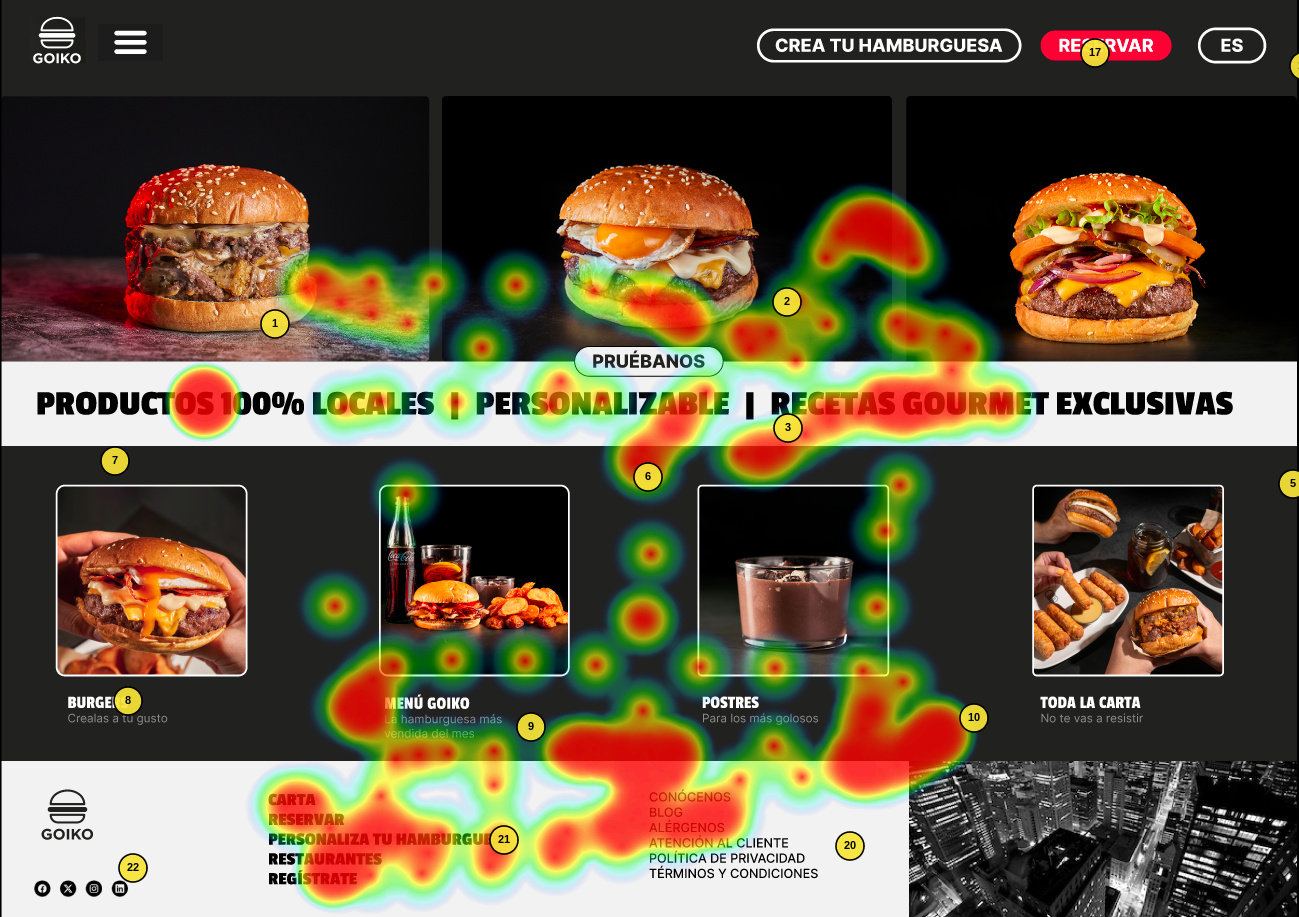
\includegraphics[width=\textwidth]{heatmapLP.jpg}
    \caption{Landing Page (Escritorio)}
  \end{subfigure}
  \hfill
  \begin{subfigure}[b]{0.38\textwidth}
    %% heatmap1: 767x4815 px — mostramos los primeros 900px (parte superior)
    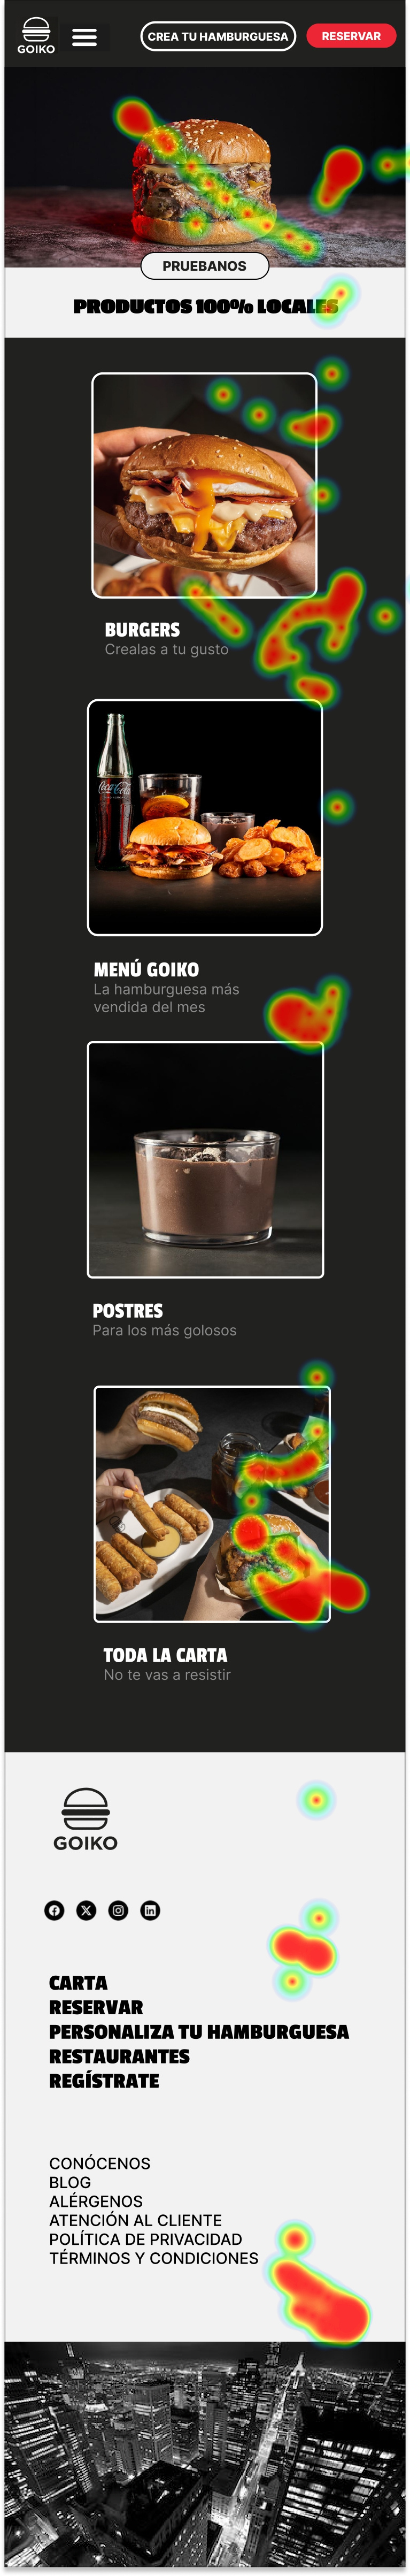
\includegraphics[width=\textwidth, viewport=0 3915 767 4815, clip]{heatmap1.jpg}
    \caption{Landing Page (Móvil — parte superior)}
  \end{subfigure}
  \caption{Mapas de calor — Landing Pages}
\end{figure}

%% ── Fila 2: Personalización (scroll largo, mostramos top 2200 px) ──
\begin{figure}[H]
  \centering
  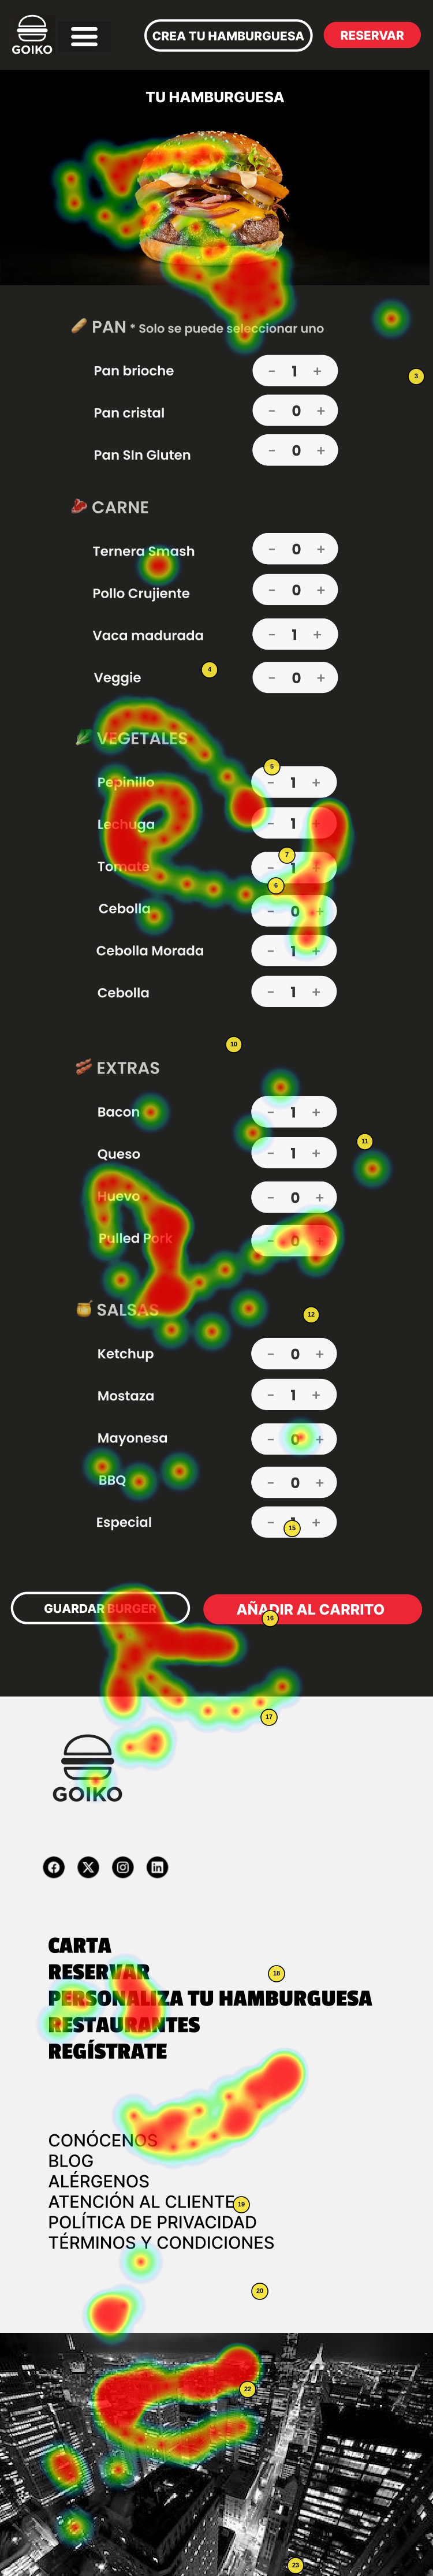
\includegraphics[width=0.27\textwidth, viewport=0 2261 750 4461, clip]{heatmap2.jpg}
  \caption{Personaliza tu Burger — zona superior (PAN, CARNE, VEGETALES, EXTRAS, SALSAS)}
\end{figure}

%% ── Fila 3: Flujo de compra (Carrito, Pago, Confirmación) ──
\begin{figure}[H]
  \centering
  \begin{subfigure}[b]{0.30\textwidth}
    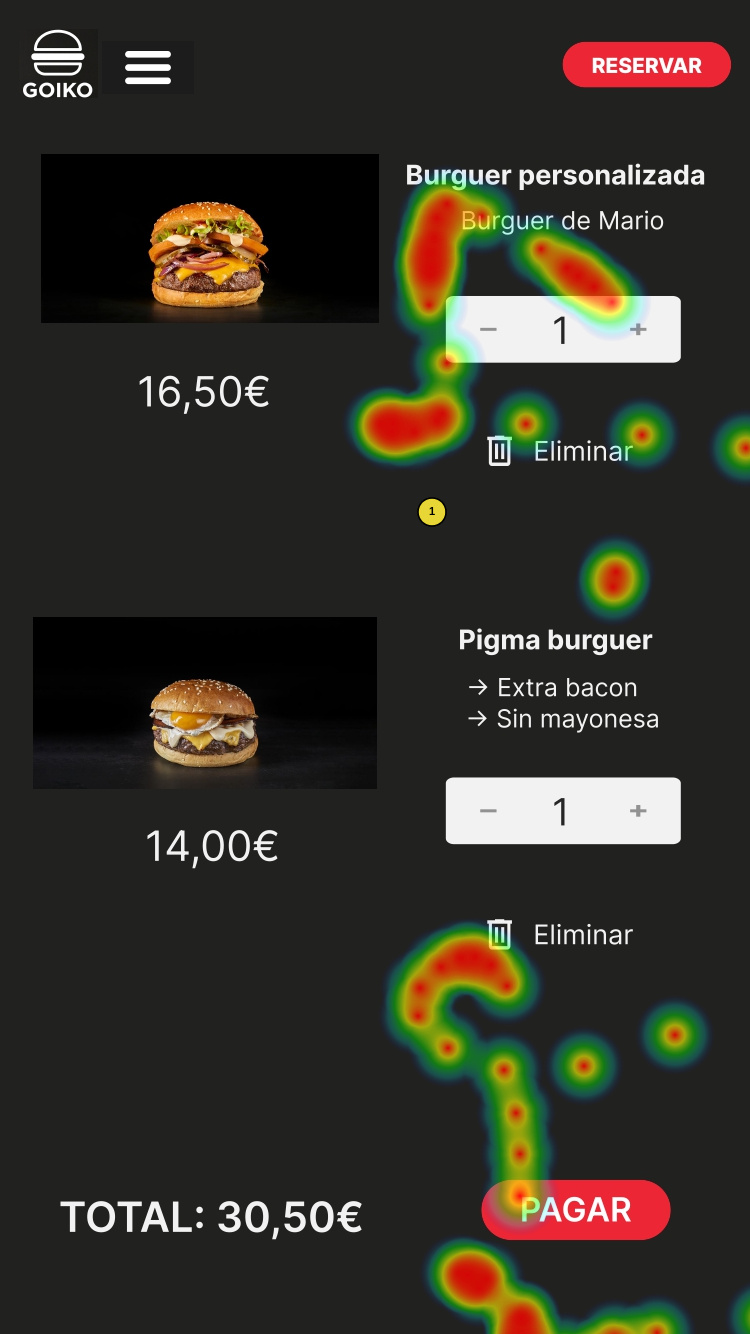
\includegraphics[width=\textwidth]{heatmap3.jpg}
    \caption{Carrito}
  \end{subfigure}
  \hfill
  \begin{subfigure}[b]{0.30\textwidth}
    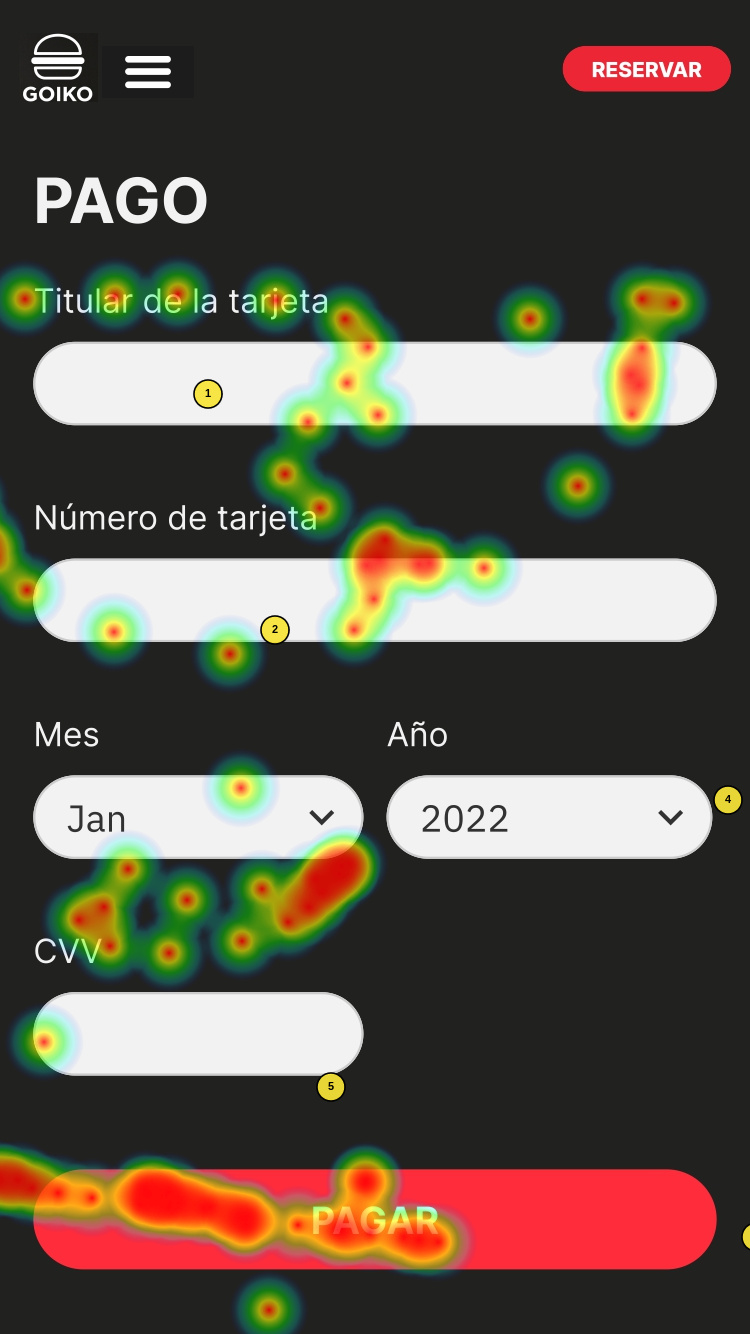
\includegraphics[width=\textwidth]{heatmap4.jpg}
    \caption{Formulario de Pago}
  \end{subfigure}
  \hfill
  \begin{subfigure}[b]{0.30\textwidth}
    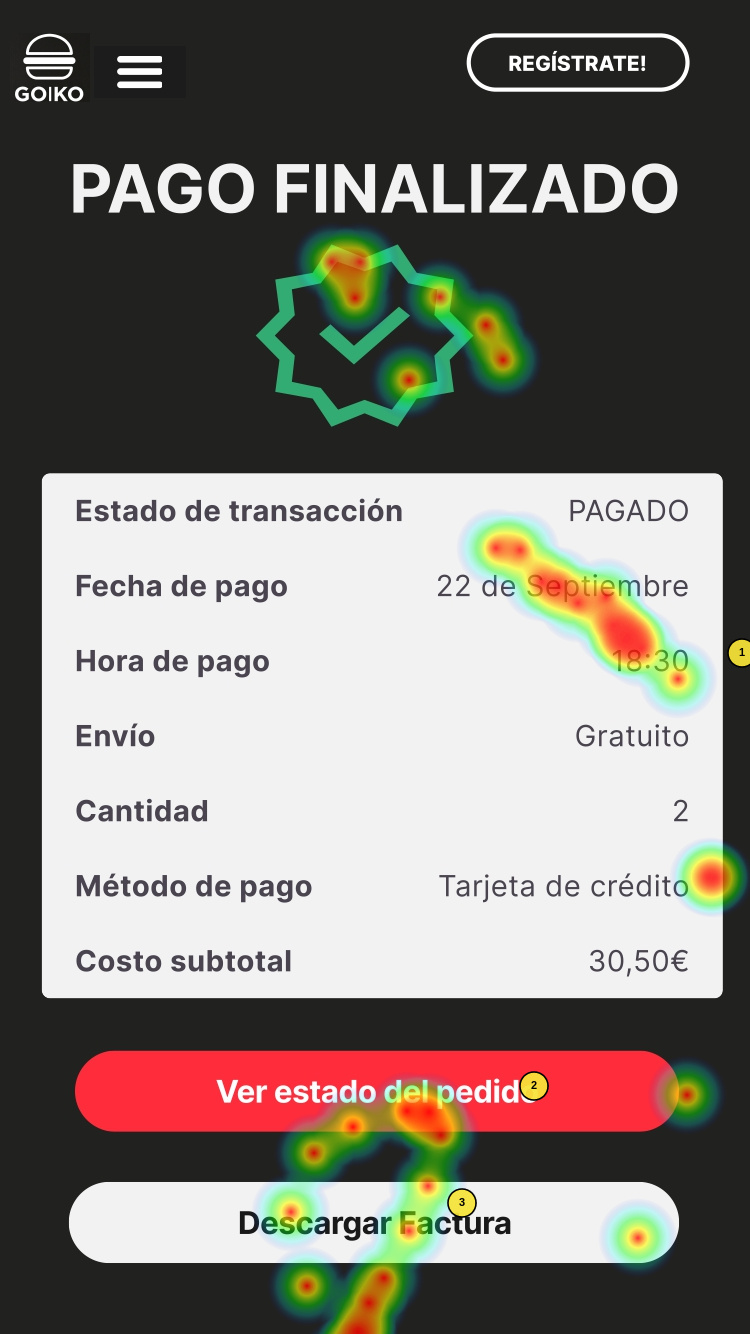
\includegraphics[width=\textwidth]{heatmap5.jpg}
    \caption{Pago Finalizado}
  \end{subfigure}
  \caption{Mapas de calor — Flujo de Compra (Carrito → Pago → Confirmación)}
\end{figure}

\subsection{Observaciones por pantalla}

\subsubsection{Landing Page}

\begin{itemize}
  \item La concentración de calor más intensa se registra en la \textbf{imagen hero central}
        y el \textbf{logotipo}. El botón principal de reserva recibe muy poca atención,
        confundiéndose visualmente con el resto de la cabecera.
  \item \textbf{Hero Section sin CTA definido:} El \textit{hero} carece de un botón de
        llamada a la acción claramente diferenciado. Los usuarios fijan la vista en la imagen
        y el texto pero no identifican ningún elemento accionable inmediato, rompiendo el
        flujo de conversión desde la primera pantalla.
  \item \textbf{Zona de silencio crítica:} El CTA de reserva —el elemento de conversión
        más importante— es ignorado por la mayoría en la primera exploración libre.
\end{itemize}

\subsubsection{Personalización de hamburguesa}

\begin{itemize}
  \item El proceso de elección de salsas generó confusión al situarse al final del flujo,
        provocando abandono parcial en los perfiles de Pilar (P08) y Nadia (P10).
  \item \textbf{Lista de opciones excesivamente larga:} El mapa de calor revela atención
        dispersa verticalmente sin anclaje en ningún elemento concreto. La ausencia de
        agrupación visual clara dificulta localizar la opción deseada y aumenta la carga
        cognitiva. Los perfiles menos técnicos muestran patrones de exploración erráticos
        que terminan en abandono parcial de la tarea.
\end{itemize}

\subsubsection{Página de Reservas y Footer}

\begin{itemize}
  \item Los usuarios exploraron el formulario de reservas de forma \textbf{errática}.
        El selector de fecha y hora no fue identificado de inmediato — varios usuarios
        lo buscaron en la zona inferior antes de encontrarlo en la superior.
  \item Los iconos de redes sociales del \textit{footer} fueron \textbf{ignorados por la
        totalidad de los usuarios}, lo que indica que no funcionan como canal de contacto
        secundario efectivo.
\end{itemize}

\begin{keybox}[Hallazgo Clave — Eye Tracking]
El \textbf{100\% de los usuarios} ignoró el botón CTA de reserva en la \textit{landing page}
durante la exploración inicial. Solo lo localizaron cuando se les indicó explícitamente la
tarea y, en algunos casos, con dificultad visible.
\end{keybox}

%% ════════════════════════════════════════════════════════════════
\section{Auditoría de Accesibilidad}
%% ════════════════════════════════════════════════════════════════

La auditoría se realizó sobre
\href{https://goikomejorado.surge.sh}{\texttt{goikomejorado.surge.sh}}
con \textbf{WAVE} y \textbf{Google Lighthouse} (escritorio y móvil).
Marco de referencia: \textbf{WCAG 2.1 nivel AA} · Norma UNE-EN 301549.

\subsection{WAVE — Web Accessibility Evaluation Tool}

\begin{figure}[H]
  \centering
  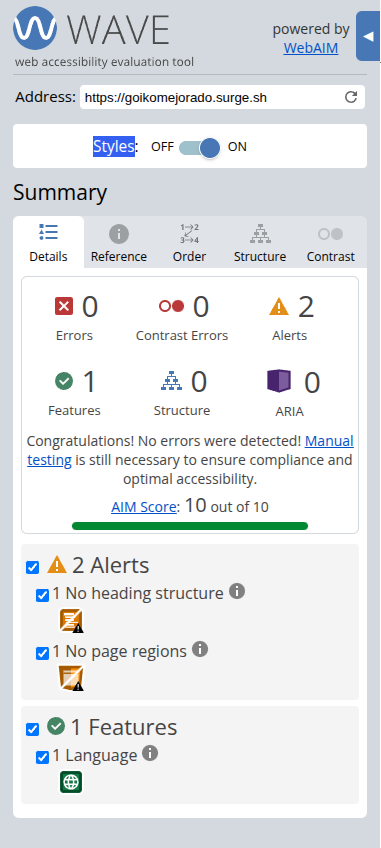
\includegraphics[width=0.72\textwidth]{wave.png}
  \caption{Resultado WAVE — 0 errores críticos · AIM 10/10 · 2 alertas estructurales}
\end{figure}

WAVE no detectó ningún error crítico ni error de contraste (\textbf{AIM 10/10}).
Sin embargo, registró \textbf{2 alertas} relevantes:

\begin{itemize}
  \item \textbf{Sin estructura de encabezados} (\textit{No heading structure}):
        ausencia de etiquetas \texttt{<h1>}, \texttt{<h2>}, \texttt{<h3>} jerárquicas.
        Impide que los usuarios de lectores de pantalla naveguen por secciones.
  \item \textbf{Sin regiones de página} (\textit{No page regions}):
        sin \textit{landmarks} semánticos (\texttt{<header>}, \texttt{<main>},
        \texttt{<nav>}, \texttt{<footer>}), dificultando la navegación por teclado
        y con tecnologías asistivas.
\end{itemize}

\textbf{Punto positivo:} el idioma de la página está correctamente declarado
(\texttt{lang="es"}), lo que permite a los lectores de pantalla pronunciar el
contenido en castellano sin configuración adicional.

\subsection{Google Lighthouse}

\begin{figure}[H]
  \centering
  \begin{subfigure}[b]{0.47\textwidth}
    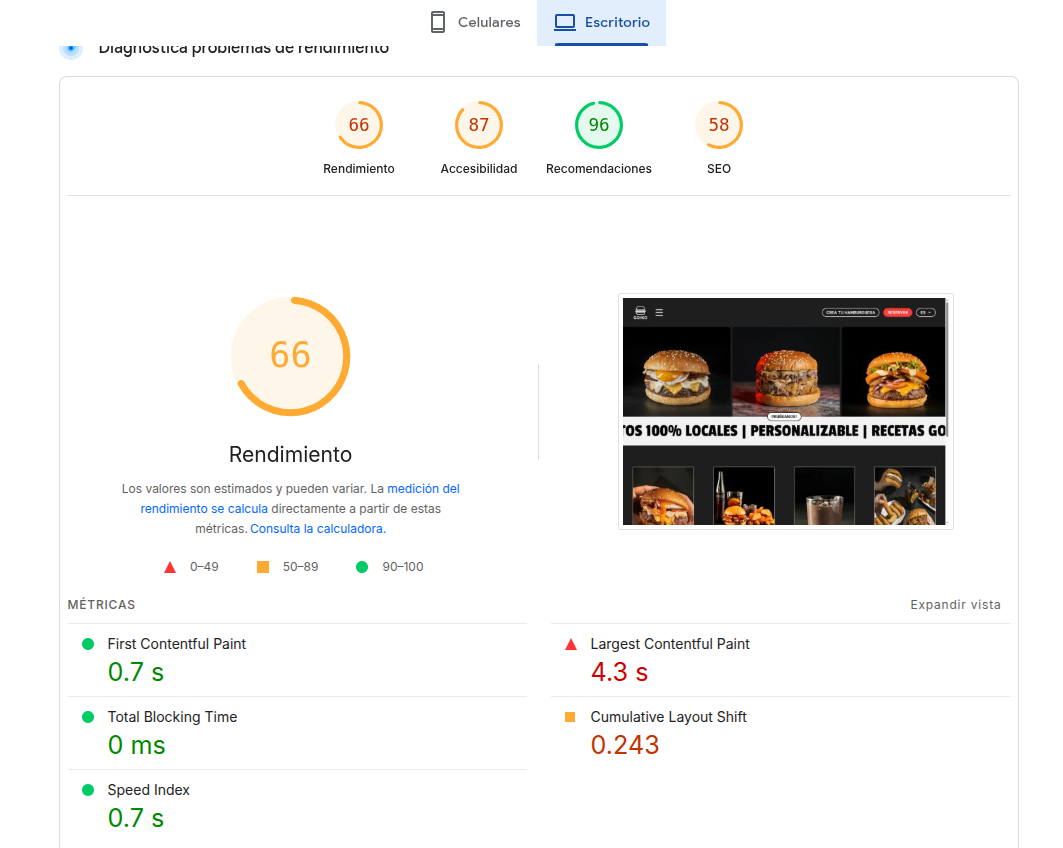
\includegraphics[width=\textwidth]{lightescritorio.png}
    \caption{Lighthouse — Escritorio}
  \end{subfigure}
  \hfill
  \begin{subfigure}[b]{0.47\textwidth}
    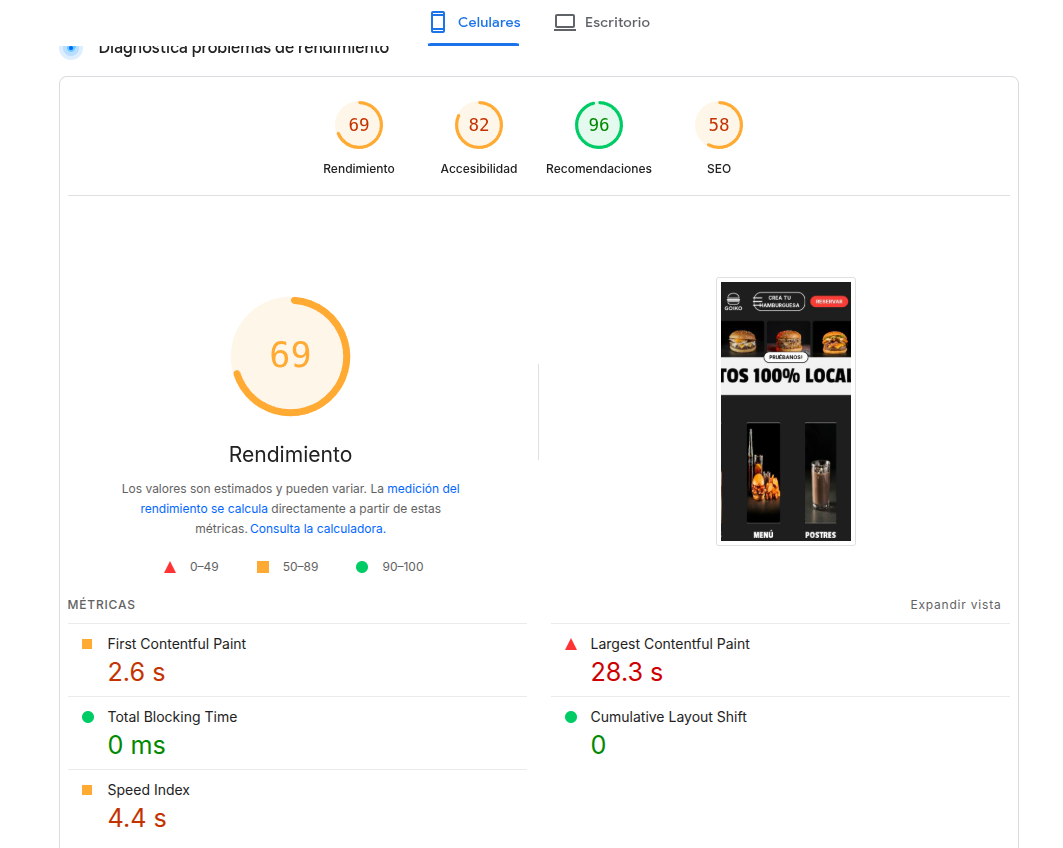
\includegraphics[width=\textwidth]{lightmovil.png}
    \caption{Lighthouse — Móvil}
  \end{subfigure}
  \caption{Google Lighthouse / PageSpeed Insights — puntuaciones por categoría}
\end{figure}

\begin{table}[H]
\centering
\caption{Puntuaciones Lighthouse — escritorio vs. móvil}
\begin{tabularx}{0.68\textwidth}{@{} X C{2.6cm} C{2.6cm} @{}}
\toprule
\rowcolor{tabhead}
\color{white}\textbf{Métrica}     &
\color{white}\textbf{Escritorio}  &
\color{white}\textbf{Móvil}       \\
\midrule
Rendimiento      &
  \textcolor{warnamber}{\textbf{66/100}}  &
  \textcolor{warnamber}{\textbf{69/100}}  \\
\rowcolor{roweven}
Accesibilidad    &
  \textcolor{okgreen}{\textbf{87/100}}    &
  \textcolor{warnamber}{\textbf{82/100}}  \\
Buenas prácticas &
  \textcolor{okgreen}{\textbf{96/100}}    &
  \textcolor{okgreen}{\textbf{96/100}}    \\
\rowcolor{roweven}
SEO              &
  \textcolor{dangerred}{\textbf{58/100}}  &
  \textcolor{dangerred}{\textbf{58/100}}  \\
\bottomrule
\end{tabularx}
\end{table}

\subsection{Análisis por principios WCAG 2.1}

\medskip
\noindent\textbf{[Perceptible — WCAG 1.3.1]}\enspace
Sin estructura de encabezados (\texttt{<h1>}, \texttt{<h2>}...)\\
\textit{Impacto:} Los usuarios con lector de pantalla no pueden identificar la jerarquía
de contenido ni navegar por secciones.\\
\textit{Recomendación:} Añadir etiquetas de encabezado semánticas y jerárquicas en
todas las secciones del documento.

\medskip
\noindent\textbf{[Perceptible — WCAG 1.4.4]}\enspace
LCP de 28,3s en móvil\\
\textit{Impacto:} Las imágenes sin optimizar bloquean la carga del contenido principal;
en conexiones estándar el usuario espera casi 30 segundos.\\
\textit{Recomendación:} Convertir imágenes a WebP, implementar \textit{lazy loading}
y definir dimensiones explícitas en los elementos visuales.

\medskip
\noindent\textbf{[Operable — WCAG 2.5.3]}\enspace
CLS de 0,243 en escritorio\\
\textit{Impacto:} El desplazamiento visual durante la carga provoca clics accidentales
en elementos incorrectos, especialmente grave para usuarios con control motor reducido.\\
\textit{Recomendación:} Reservar espacio explícito (\texttt{width}/\texttt{height})
en todos los elementos de imagen cargados de forma asíncrona.

\medskip
\noindent\textbf{[Comprensible — WCAG 1.3.6]}\enspace
Sin regiones de página (\texttt{<main>}, \texttt{<nav>}, \texttt{<footer>})\\
\textit{Impacto:} La navegación por teclado o lector de pantalla carece de puntos de
referencia semánticos para saltar al contenido principal.\\
\textit{Recomendación:} Añadir \textit{landmarks} HTML5 semánticos en todos los
bloques estructurales de la página.

\medskip
\noindent\textbf{[Robusto — WCAG 4.1.1]}\enspace
SEO 58/100; sin metadatos estructurados ni etiquetas semánticas\\
\textit{Impacto:} Agentes de usuario y tecnologías asistivas no pueden interpretar
correctamente la estructura del documento.\\
\textit{Recomendación:} Añadir \texttt{<title>}, \texttt{<meta description>},
\texttt{aria-label} en elementos interactivos y datos estructurados JSON-LD.

\begin{infobox}
\textbf{Valoración global de accesibilidad: 6/10} — Cumple los mínimos técnicos
(0 errores de contraste, buenas prácticas 96/100) pero requiere mejoras estructurales
y de rendimiento para alcanzar el nivel AA completo. El LCP de 28,3s en móvil
es la barrera más crítica.
\end{infobox}

%% ════════════════════════════════════════════════════════════════
\section{Conclusiones y Recomendaciones}
%% ════════════════════════════════════════════════════════════════

\subsection{Resultados del A/B Testing}

\begin{table}[H]
\centering
\caption{Resultados de las tareas — Mejora de Goiko (Caso B)}
\begin{tabularx}{\textwidth}{@{} X C{2cm} C{2.5cm} C{2.5cm} @{}}
\toprule
\rowcolor{tabhead}
\color{white}\textbf{Tarea}               &
\color{white}\textbf{\% Éxito}            &
\color{white}\textbf{T. medio}            &
\color{white}\textbf{Clics medios}        \\
\midrule
Pedir una hamburguesa               &
  \textcolor{dangerred}{\textbf{60\%}} & 38s & 5 \\
\rowcolor{roweven}
Elegir salsas extra                 &
  80\% & 20s & \textcolor{warnamber}{\textbf{9}} \\
Realizar pago y rellenado de datos  &
  80\% & \textcolor{dangerred}{\textbf{78s}} & 4 \\
\rowcolor{roweven}
Encontrar contacto y redes sociales &
  \textcolor{okgreen}{\textbf{100\%}} & 18s & 3 \\
\midrule
\rowcolor{tabhead}
\color{white}\textbf{Media general} &
\color{white}\textbf{80\%}          &
\color{white}\textbf{38,5s}         &
\color{white}\textbf{5}             \\
\bottomrule
\end{tabularx}
\end{table}

\begin{infobox}
\textbf{Valoración general media (escala 1–7):}\enspace
Caso B: \textbf{4,0 / 7}\enspace·\enspace
Caso A (referencia): \textit{4,8 / 7}
\end{infobox}

\subsection{Recomendaciones priorizadas}

\noindent\textbf{[Alta — Crítica]}\enspace
El CTA de reserva en la \textit{Landing Page} es ignorado por el 100\% de usuarios.\\
\textit{Mejora:} Aumentar contraste, tamaño y posición del botón; añadir un elemento
gráfico diferenciador sobre el hero con color de alto contraste.

\medskip
\noindent\textbf{[Alta — Crítica]}\enspace
El flujo de reserva/pago tarda 78s de media y genera abandono en perfiles con bajo nivel digital.\\
\textit{Mejora:} Reducir campos visibles en la primera pantalla; dividir el proceso en pasos
numerados con indicador de progreso.

\medskip
\noindent\textbf{[Alta — Crítica]}\enspace
LCP de 28,3s en móvil — el sitio no carga a tiempo en conexiones estándar.\\
\textit{Mejora:} Comprimir imágenes a WebP, implementar \textit{lazy loading} y caché de
recursos estáticos.

\medskip
\noindent\textbf{[Media]}\enspace
Sin estructura de encabezados ni \textit{landmarks} HTML5 semánticos.\\
\textit{Mejora:} Añadir jerarquía de \textit{headings} y \textit{landmarks} para cumplir
WCAG 2.1 AA.

\medskip
\noindent\textbf{[Media]}\enspace
La sección de elección de salsas está al final del flujo: 9 clics medios y abandono parcial.\\
\textit{Mejora:} Reposicionar la personalización antes del carrito; agrupar opciones
visualmente por categoría.

\medskip
\noindent\textbf{[Media]}\enspace
CLS de 0,243 en escritorio provoca clics accidentales durante la carga.\\
\textit{Mejora:} Reservar espacio explícito (\texttt{height}/\texttt{width}) en los
elementos de imagen asíncronos.

\medskip
\noindent\textbf{[Baja]}\enspace
Los iconos de redes sociales del \textit{footer} son ignorados por todos los usuarios.\\
\textit{Mejora:} Acompañar los iconos con etiquetas de texto o moverlos a una zona
más visible de la página.

\medskip
\noindent\textbf{[Baja]}\enspace
SEO 58/100 — falta de metaetiquetas y etiquetas semánticas.\\
\textit{Mejora:} Añadir \texttt{<title>}, \texttt{<meta description>},
\texttt{aria-label} y datos estructurados JSON-LD.

\subsection{Valoración final del equipo evaluador}

El diseño de Mejora de Goiko presenta una propuesta visual moderna y atractiva, especialmente
bien valorada por perfiles con alta competencia digital (Elena, David). La arquitectura general
es comprensible y el flujo de contacto funciona correctamente (100\% de éxito, 18s).

Sin embargo, la usabilidad se resiente significativamente cuando el usuario tiene un perfil
menos técnico o accede desde móvil. El cuello de botella principal es el proceso de
reserva/pedido: demasiados pasos, tiempo excesivo (78s) y un CTA invisible en la pantalla
de entrada. Estos problemas explican la puntuación SUS de 62,0 (Marginal) y la diferencia
de 11 puntos frente al Caso A.

\begin{keybox}[Conclusión Final]
Con las mejoras propuestas en prioridad \textbf{Alta}, el diseño podría alcanzar un rango
\textbf{«Bueno» (SUS $>$ 70)} y cumplir los requisitos mínimos de accesibilidad
\textbf{WCAG 2.1 AA}, convirtiéndose en una base sólida para producción.
\end{keybox}

\vspace{2.5em}
\noindent{\color{goikored}\rule{\textwidth}{1pt}}
\vspace{0.4em}

\begin{center}
  \small\color{medgray}
  Informe elaborado por el equipo \textbf{DIU2.Errores404}\\
  Asignatura Diseño de Interfaces de Usuario ·
  Universidad de Granada · Curso 2025/26
\end{center}

\end{document}
